Obrazy testowe, które nazwane są tutaj danymi zewnętrznymi, są rysunkami grafów pochodzącymi spoza przygotowanego testu.
Dzielą się na obrazy pobrane z internetu, obrazy wygenerowane przez skrypt w R, ale nie używane w treningu,
oraz rysunki odręczne grafów. Typy danych zewnętrznych wybiegają poza klasy grafów wykorzystywanych przy uczeniu modelu.

\begin{figure}[ht]
	\centering
	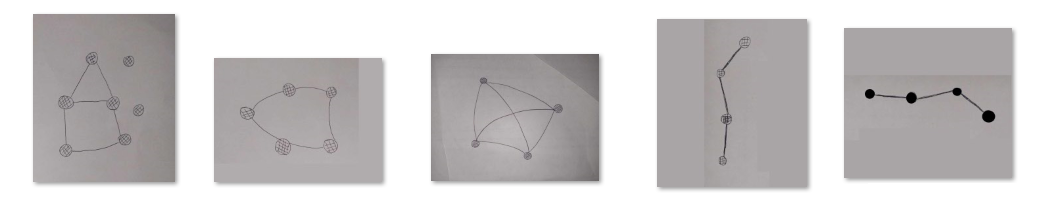
\includegraphics[width=15.5cm]{resources/tests/images/ext-graphs-drawn.png}
	\caption{Przykładowe zewnętrzne rysunki grafów narysowane odręcznie}
	\label{Fig:tests-outside-1}
\end{figure}
\FloatBarrier

\begin{figure}[ht]
	\centering
	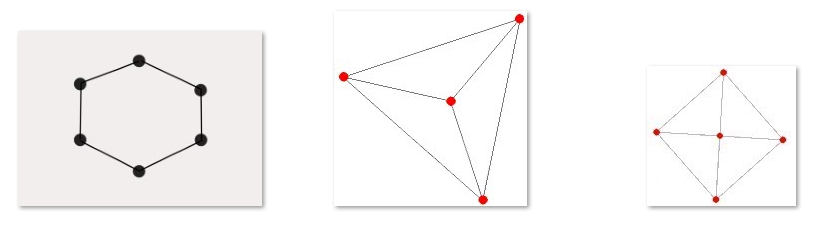
\includegraphics[width=15cm]{resources/tests/images/ext-graphs-internet.png}
	\caption{Przykładowe zewnętrzne rysunki grafów pobrane z internetu}
	\label{Fig:tests-outside-2}
\end{figure}
\FloatBarrier